% The first argument is the \documentclass, which tells latex which template
% we're using to build this document. It's usually safe to just use "article".
\documentclass{article}

% include some packages...
\usepackage{fullpage} % change settings for a smaller margin
\usepackage{graphicx} % gives access to the \includegraphics commands
\usepackage{amsfonts}
\usepackage{float}
\usepackage{enumitem}
\usepackage{caption}
\usepackage[export]{adjustbox}
\usepackage{bookmark}
\graphicspath{{./images/}}

% tell Latex to use no paragraph indentation, but leave some space between
% paragraphs 
\setlength{\parindent}{0in}
\setlength{\parskip}{0.1in}

\newcommand{\tib}[1]{\textit{\textbf{#1}}}
\newcommand{\code}[1]{\texttt{#1}}

% these commands merely set the values for the title/date/author; they don't put
% them in the document... see \maketitle below
\title{CS Department Automated Information Timeline \\ Assignment 3.1: Domain Model}
\date{\today}
\author{Matthew Hays, Pawan Bhandari, Sarah Faron, Tim Klimpel}

% all document content goes between \begin{document} and \end{document}
\begin{document}

% this command actually creates the title/date/author in the document
\maketitle
\newpage
\tableofcontents
\listoffigures
\newpage

\section{Introduction}
\subsection{Purpose}
The purpose of this assignment is to work as a team and collaboratively develop a final Domain model for the group project.  The team met multiple times over the course of a few days to work together and come to the final model presented in the third section of this document (Located here: \nameref{fig:FinalDomain}).

\subsection{Background from Readings}\label{sec:readings}
According to C. Larman, The three strategies to identify candidate concepts are:
\begin{itemize}
    \item Noun-Phrase Identification from use cases and requirements
    \item Conceptual Class Category Lists
    \item Class Responsibility Collaborators
\end{itemize}
The concepts on the domain model for CS Department Automated Information Timeline project have been derived by identifying the noun phrases from use cases and the requirements.

\section{Concepts, Attributes, and Associations (Draft)}
Below are the candidate concepts and their attributes identified using the noun phrases from the requirements.

\vspace{2ex}
\begin{minipage}{0.325\textwidth}
    \begin{enumerate}
        \item \textbf{Post}: title, content
        \item \textbf{DisplayedPost}
        \item \textbf{Page}: title, content
        \item \textbf{Event}: dateOfEvent
        \item \textbf{EventCalender}
        \item \textbf{Media}: title, mediatype
        \item \textbf{MediaLibrary}
        \item \textbf{Notification}
        \item \textbf{Faculty}: name
        \item \textbf{OfficeManager}: name
        \item \textbf{Administrator}
        \item \textbf{DisplayedMedia}
        \item \textbf{DisplayMonitor}
    \end{enumerate}
\end{minipage}
%
\begin{minipage}{0.65\textwidth}
    \begin{figure}[H]
        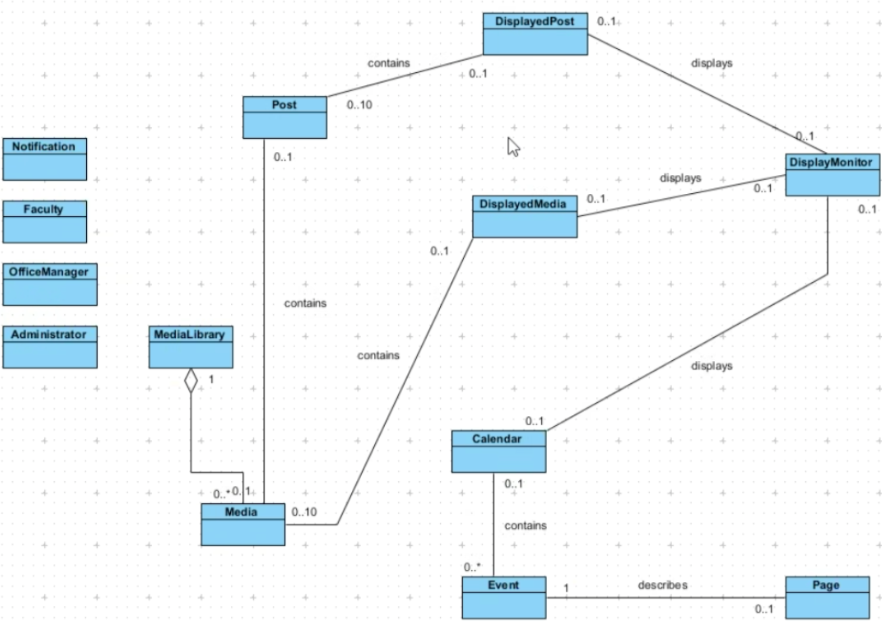
\includegraphics[width=.9\textwidth,right]{./draft-Concepts.png}
        \caption{Candidate concepts and associations (Draft)}
        \label{fig:canidate}
    \end{figure}
\end{minipage}

\vspace{2ex}
These candidate concepts are further discussed among the team members and are further refined to create a \textbf{FINAL DOMAIN MODEL} with concepts, name associations and multiplicities agreed upon by all team members.

\section{Domain Model}
\subsection{Domain Model (Drafts)}
\begin{figure}[H]
    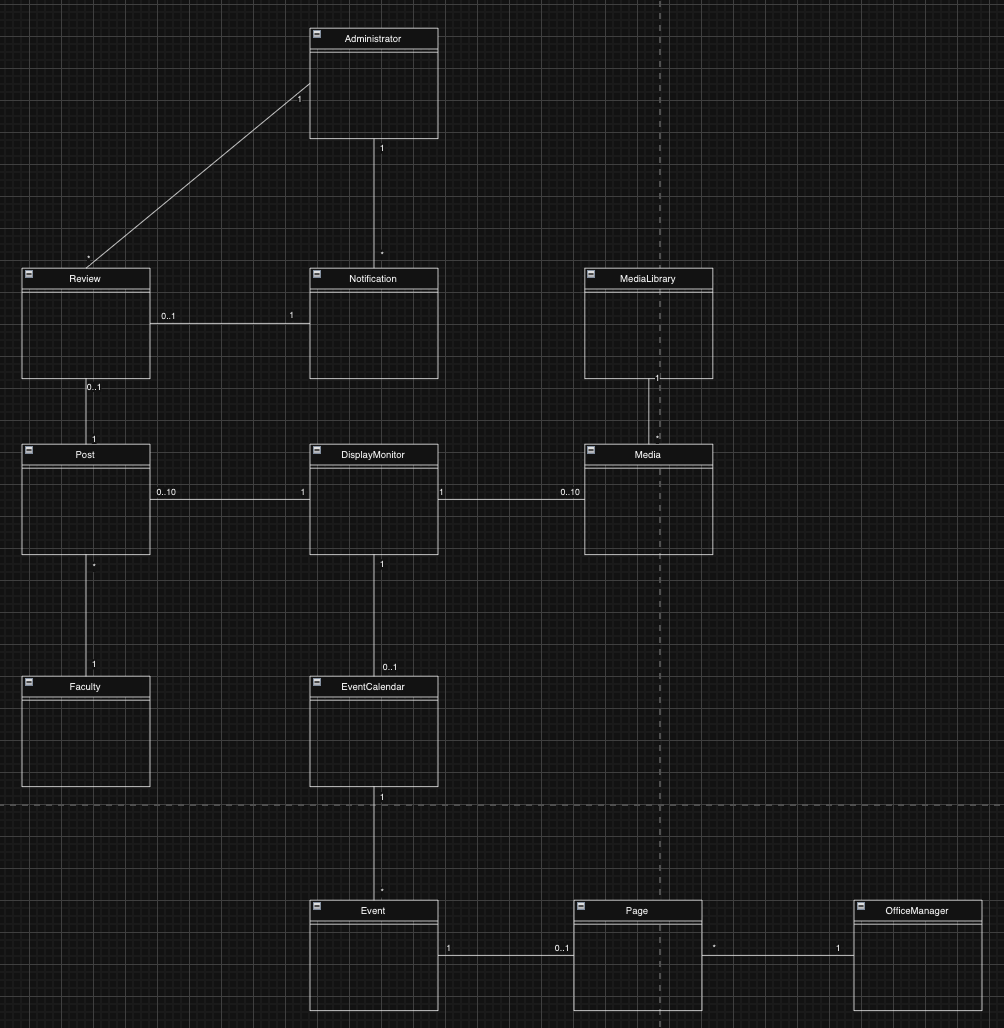
\includegraphics[width=.9\textwidth]{./Initial Domain Model.png}
    \centering
    \caption{Domain Model - Draft 1}
    \label{fig:DraftDomainv1}
\end{figure}

\begin{figure}[H]
    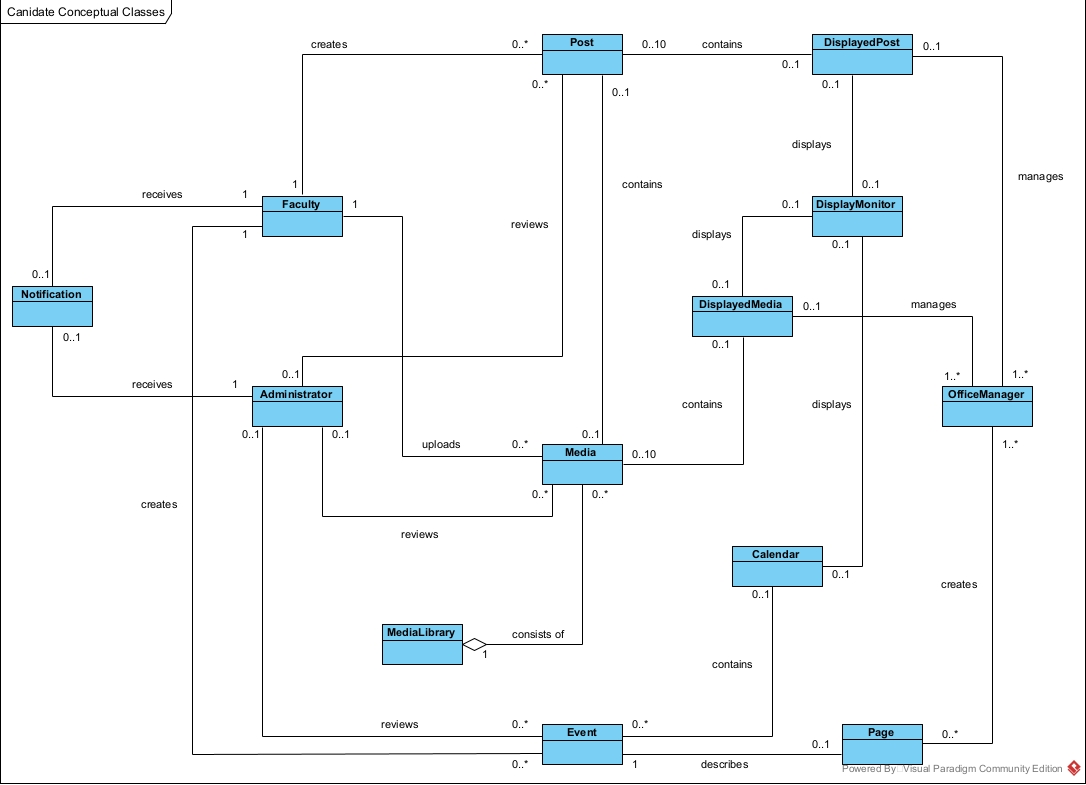
\includegraphics[width=.9\textwidth]{./draft-DomainModel.jpg}
    \centering
    \caption{Domain Model - Draft 2}
    \label{fig:DraftDomainv2}
\end{figure}

\subsection{Getting to the Final Domain Model}
\subsubsection{Use Case text reference}
Below are the summarized use cases.  This listing has been updated from the previous design submittal, and an updated use case diagram can be found at the end of this document.  New use cases found are flagged in list as well for clarity.

\vspace{2ex}
\begin{itemize}
    \item UC01 - View Media Library
    \item UC02 - View All Posts
    \item UC03 - View Event Calendar
    \item UC04 - Create Event
    \item UC05 - Edit Event
    \item UC06 - Delete Event
    \item UC07 - View Event
    \item UC08 - Submit for post/media/event review
    \item UC09 - Review for post/media/event approval
    \item UC10 - Create Post
    \item UC11 - Edit Post
    \item UC12 - Delete Post
    \item UC13 - View Post
    \item UC15 - Stage posts for display
    \item UC16 - Stage media for display
    \item UC17 - View Media
    \item UC18 - Add Page to Event \textit{(New Use Case)}
    \item UC19 - Edit Page of Event \textit{(New Use Case)}
    \item UC20 - Tag Event for display \textit{(New Use Case)}
    \item UC21 - Receive notification for approval request \textit{(New Use Case)}
    \item UC22 - Receive notification for approval completion \textit{(New Use Case)}
    \item UC23 - Upload new Media \textit{(New Use Case)}
    \item UC24 - Send Notifications for approval request/completions \textit{(New Use Case)}
\end{itemize}
% \subsection{Notes on Domain Model drafts}
% The domain model draft had the concept of "Displayed Media" and "Displayed post" which were managed by the office manager but the team decided in favor of office manager staging the posts and media directly since it was the core responsibility of the office manager as outlined in the project requirements. This also seemed to align with the idea that the Domain model is meant to represent real world objects, and the agreeded upon thought was that the Post and Media items themselves would be responsible for knowing if they were staged or not.

% The requirement that the TV display only displays 10 most recent posts/media is represented by the 0...10 multiplicity in the "displays" association between the post and media and the DisplayMonitor.

% The system will impose a limit of 10 on the number of posts and media that can be staged for display by a office manager. In the event of multiple Office Managers, 10 tagged/staged media or posts will be selected for display to maintain a limit of 10 items in a specific category being displayed at any given time on the DisplayMonitor.

% The concept of a Media Library was included as an aggregation of media so that users can browse the approved media(photos and videos) as opposed to media items being locked down to only be included as part of Post items.

% Upon creation of any category of item submitted to the application, the new item will be initially set to a state which does not allow for display/inclusion in the application. This state can only be updated through a review by a system administrator, as captured by the "reviews" association from Administrator to the relevant item (Post/Media/Event).

\subsubsection{Points discussed during review of Domain model drafts}

This section contains items discussed as a group during the review and finalization of the \nameref{fig:FinalDomain}. Progression was made from \nameref{fig:DraftDomainv1} to \nameref{fig:DraftDomainv2}, but there was back and forth between the two.

% \subsubsection{Number of items to display}
\begin{itemize}
    \item The system will always display 10 of each of the following items (References \textbf{REQ10})
          \subitem$\circ$ Posts
          \subitem$\circ$ Media
          \subsubitem$\diamond$ If there are not 10 items of a particular category within the system that is in the approved state, the system will display all approved items within that category. (\textbf{Assumption based on implication in problem statement})
    \item The system will only display the event pages that have been tagged, without limit. (References \textbf{UC20, REQ18})
    \item An Office Manager can tag and/or stage up to 10 items for display at any time. (References \textbf{Assumption based on implication in problem statement}) (References \textbf{REQ10})
          \subitem$\circ$ In the event of multiple Office Managers, the system will randomly select 10 tagged/staged media for display to maintain a limit of 10 items in a specific category being displayed at any given time on the on-campus television display.
    \item An aggregate media library should exist so that users of the application may browse all approved media. (References \textbf{REQ04/REQ05/REQ09})
    \item Upon creation of any category of item submitted to the application, the new item will be initially set to a state which does not allow for display/inclusion in the application. This state can only be updated through a review by a system administrator. (References \textbf{REQ02/UC08/UC09})
    \item DisplayedMedia and DisplayedPosts were removed from the initial draft as these classes were decided to be “software constructs” that were not necessary in the domain model. Additionally, their removal assisted in the discovery that the classes may not be necessary as the intent of the classes, to provide a storage location for displayed items, could be captured through attributes located on the parent class itself. (No associated REQ or UC – software design/implementation discussion)
\end{itemize}

\subsubsection{Final Domain Model}
\begin{figure}[H]
    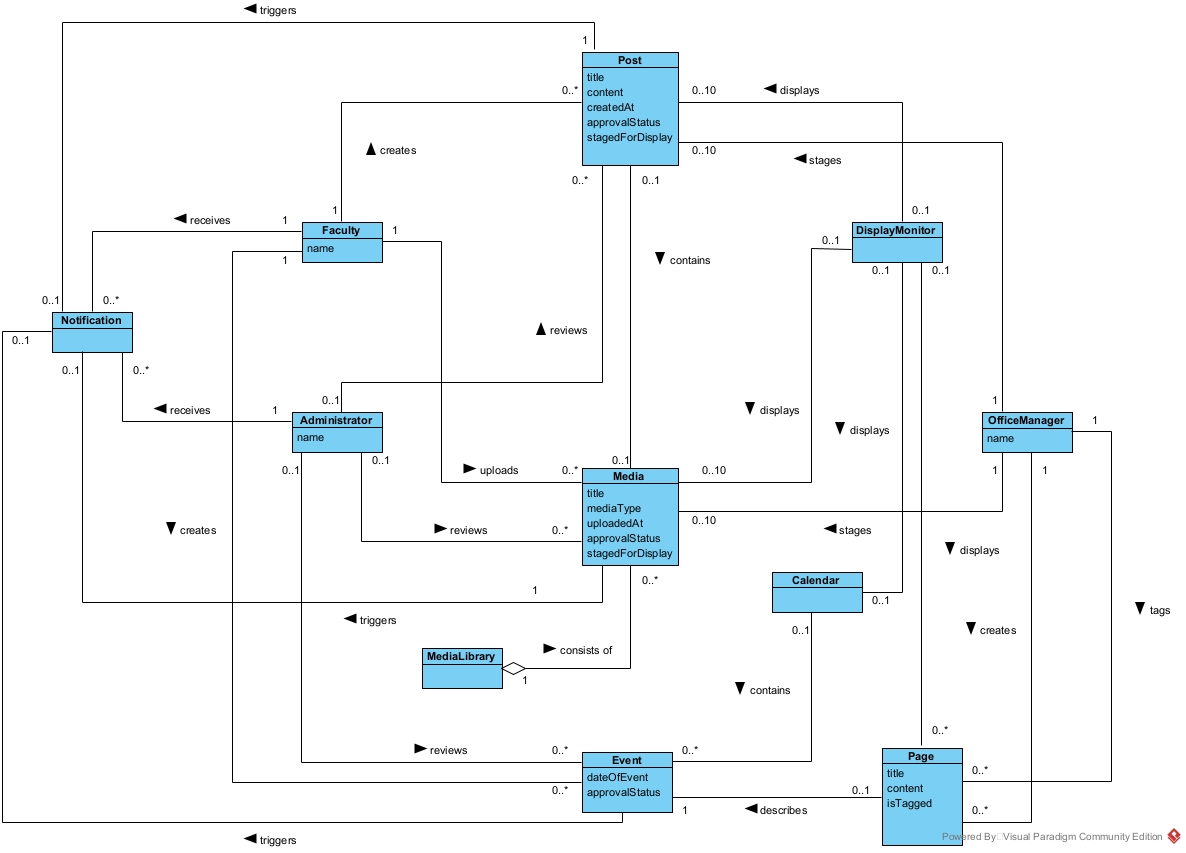
\includegraphics[width=.9\textwidth]{images/DomainModel.jpg}
    \centering
    \caption{Final Domain Model}
    \label{fig:FinalDomain}
\end{figure}
\section{Updated Use Case Diagram}
\begin{figure}[H]
    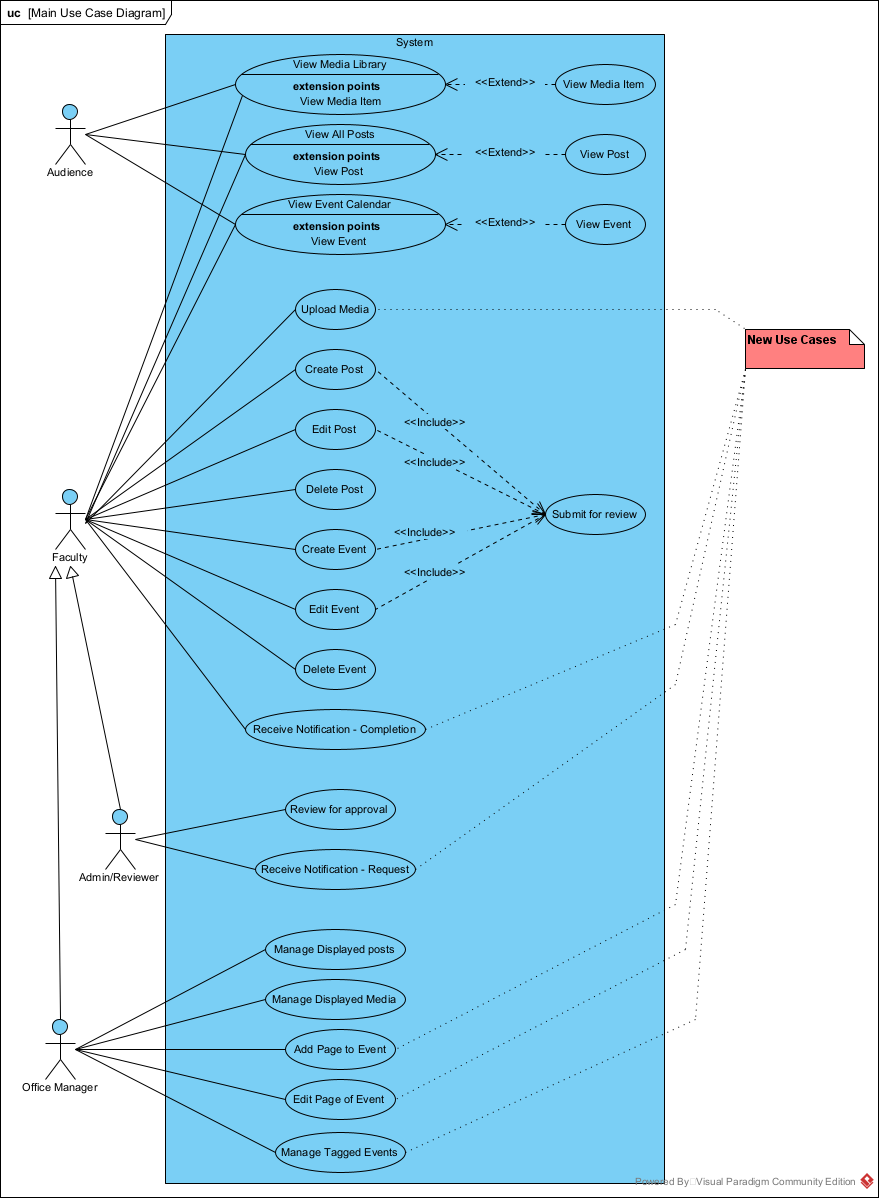
\includegraphics[width=.88\textwidth]{updatedUseCaseDiagram.png}
    \centering
    \caption{Updated Use Case Diagram}
    \label{fig:updatedUseCaseDiagram}
\end{figure}


\end{document}